%
% This is the LaTeX template file for lecture notes for CS294-8,
% Computational Biology for Computer Scientists.  When preparing 
% LaTeX notes for this class, please use this template.
%
% To familiarize yourself with this template, the body contains
% some examples of its use.  Look them over.  Then you can
% run LaTeX on this file.  After you have LaTeXed this file then
% you can look over the result either by printing it out with
% dvips or using xdvi.
%
% This template is based on the template for Prof. Sinclair's CS 270.

\documentclass[11pt, twosides]{article}
\usepackage[utf8]{inputenc}
\usepackage{hyperref}
\usepackage{graphicx}
\usepackage{graphics}
\usepackage{amsmath}
\usepackage{amsfonts}
\usepackage{amssymb}
\usepackage{amsthm}
\usepackage{xcolor}
\setlength{\oddsidemargin}{0.25 in}
\setlength{\evensidemargin}{-0.25 in}
\setlength{\topmargin}{-0.6 in}
\setlength{\textwidth}{6.5 in}
\setlength{\textheight}{8.5 in}
\setlength{\headsep}{0.75 in}
\setlength{\parindent}{0 in}
\setlength{\parskip}{0.1 in}

%
% The following commands set up the lecnum (lecture number)
% counter and make various numbering schemes work relative
% to the lecture number.
%
\newcounter{lecnum}
\renewcommand{\thepage}{\thelecnum-\arabic{page}}
\renewcommand{\thesection}{\thelecnum.\arabic{section}}
\renewcommand{\theequation}{\thelecnum.\arabic{equation}}
\renewcommand{\thefigure}{\thelecnum.\arabic{figure}}
\renewcommand{\thetable}{\thelecnum.\arabic{table}}

%
% The following macro is used to generate the header.
%
\newcommand{\lecture}[4]{
%   \pagestyle{myheadings}
   \thispagestyle{plain}
   \newpage
   \setcounter{lecnum}{#1}
   \setcounter{page}{1}
   \noindent
   \begin{center}
   \framebox{
      \vbox{\vspace{2mm}
    \hbox to 6.28in { {\bf CS 419M Introduction to Machine Learning
                        \hfill Spring 2021-22} }
       \vspace{4mm}
       \hbox to 6.28in { {\Large \hfill Lecture #1: #2  \hfill} }
       \vspace{2mm}
       \hbox to 6.28in { {\it Lecturer: #3 \hfill Scribe: #4} }
      \vspace{2mm}}
   }
   \end{center}
   \markboth{Lecture #1: #2}{Lecture #1: #2}
}

%
% Convention for citations is authors' initials followed by the year.
% For example, to cite a paper by Leighton and Maggs you would type
% \cite{LM89}, and to cite a paper by Strassen you would type \cite{S69}.
% (To avoid bibliography problems, for now we redefine the \cite command.)
% Also commands that create a suitable format for the reference list.
% \renewcommand{\cite}[1]{[#1]}
% \def\beginrefs{\begin{list}%
%         {[\arabic{equation}]}{\usecounter{equation}
%          \setlength{\leftmargin}{2.0truecm}\setlength{\labelsep}{0.4truecm}%
%          \setlength{\labelwidth}{1.6truecm}}}
% \def\endrefs{\end{list}}
% \def\bibentry#1{\item[\hbox{[#1]}]}

%Use this command for a figure; it puts a figure in wherever you want it.
%usage: \fig{NUMBER}{SPACE-IN-INCHES}{CAPTION}
% \newcommand{\fig}[3]{
% 			\vspace{#2}
% 			\begin{center}
% 			Figure \thelecnum.#1:~#3
% 			\end{center}
% 	}
% Use these for theorems, lemmas, proofs, etc.
\newtheorem{theorem}{Theorem}[lecnum]
\newtheorem{lemma}[theorem]{Lemma}
\newtheorem{proposition}[theorem]{Proposition}
\newtheorem{claim}[theorem]{Claim}
\newtheorem{corollary}[theorem]{Corollary}
\newtheorem{definition}[theorem]{Definition}
% \newenvironment{proof}{{\bf Proof:}}{\hfill\rule{2mm}{2mm}}

% **** IF YOU WANT TO DEFINE ADDITIONAL MACROS FOR YOURSELF, PUT THEM HERE:

\begin{document}
%FILL IN THE RIGHT INFO.
%\lecture{**LECTURE-NUMBER**}{**DATE**}{**LECTURER**}{**SCRIBE**}
\lecture{16}{Introduction to Deep Learning}{Dr. Ashish Tendulkar (guest)}{Group 1}
%\lecture{x}{Title}{Abir De}{Group y}

\section{Introduction to Deep Leaning}

Deep Learning also called as Artificial Neural Networks, Deep Networks, Multi-layer Preceptrons (MLP) is a machine learning model like Linear Regression, Logistic Regression, Decision Trees, SVMs .


Deep Learning Models are ML models only.   
  
\begin{itemize}
    \item \textbf{What is Machine Learning? What is the difference between Programming and ML?}
    \begin{itemize}
        \item Programming: When process is simple with given data and specified rules to obtain output. example, adding of two numbers. Writing a code to detect human faces in an image is difficult by this approach cause of brittle rules. 
       \begin{figure}[htp]
    \centering
    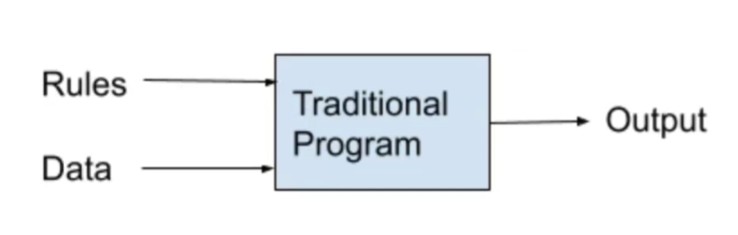
\includegraphics[width=9cm]{pr.png}
    \caption{Programming Flow Chart}
    \label{fig:galaxy}
\end{figure}
        
        \item {Machine Learning: When rules are not well defined, are brittle and its difficult to write the program in the traditional way. We have ML to the rescue.}
             \begin{figure}[htp]
    \centering
    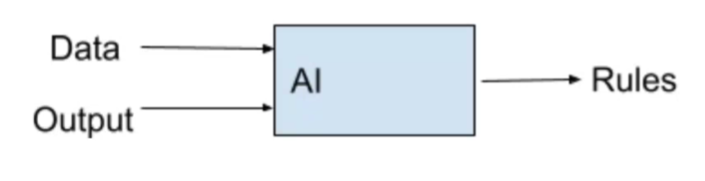
\includegraphics[width=9cm]{ml.png}
    \caption{ML Flow Chart}
    \label{fig:galaxy}
\end{figure}
\begin{itemize}
       \item We provide training data for the task at hand - Detecting human faces from the images. 
       \item Training data is in the form of input image and output binary. like (image1,label1), (image2,label2) --- (imagen,labeln)
       \item Let's say image is of pixel 32*32 than input (x) is a vector of length 1024
       \item Output (y) is a binary 
       \item Training data gives us the weights of the models. (where models are specified)
       \item After training we get inference which takes the weights and input data to give output similar to the traditional program.
        \end{itemize}
     \end{itemize}
\end{itemize}

\section{Components of ML}

Neural Network (NN) is just another machine learning concept. They also have $5$ components:

\begin{itemize}
    \item Training data (consists of features and labels) :
    \begin{itemize}
        \item Regression: training data is of the form $\left(\Vec{X_i}, y_i \right)$, where $y_i \in \mathbb{R}$. If only one label $\rightarrow$ single output, otherwise $\rightarrow$ multi-output.
        \item Classification: training data is of the form $\left(\Vec{X_i}, y_i \right)$, where $y_i \in$ a discrete set. Within classification we have binary(single label) and multiclass classification(multi-label).
    \end{itemize}
    
    \item Model:
    \begin{itemize}
        \item Linear Regression: $y=w^T x$
        \item Logistic Regression: $y=sigmoid(w^T x)$
        \item Decision Trees: Tree (By traversing the tree we can reach leaf node of the tree and based on the label in leaf node we can assign the label)
    \end{itemize}
    
    \item Loss functions:
    \begin{itemize}
        \item Regression: MSE (Mean Squared Error) loss :- \begin{equation*}\begin{split}J(w)&=\frac{1}{2}\sum_{i=1}^{n}(prediction - actual\,label)^2\\
        &=\frac{1}{2}\sum_{i=1}^{n}(w^T x - y)^2\\
        &=\frac{1}{2}(Xw - y)^T(Xw - y)\end{split}\end{equation*}
        \item Classification:  Cross Entropy loss:- $J(w)=\sum_{i=1}^{n}(actual\,label)\, log(predicted \,value)$
    \end{itemize}
    
    \item Optimization procedure
    \begin{itemize}
        \item Update rules
        \item Gradient descent, batch gradient descent, Stochastic Gradient Descent (SGD) and Greedy method for trees

    \end{itemize}
    
    \item Model selection and evaluation
    \begin{itemize}
        \item Hyper-parameter tuning (HPT): For HPT, we can use grid search, randomized search.\begin{itemize}
        \item Regularized LSE:- $J(w) = J(w) + \lambda* Penalty$\\
        Vary value of $\lambda = (1e^{-4},1e^{-3},1e^{-2},1e^{-1},0,1)$\\
        $(\lambda,MSE)\rightarrow Select\, \lambda$ that gives best MSE(calculation done on validation set)
        \item The only difference between both the approaches is in grid search we define the combinations and do training of the model whereas in Randomized Search the model selects the combinations randomly.
        \end{itemize}
        \item Metrics:\begin{itemize}\item Regression: MSE, MAE
        \item Classification: Accuracy,Precision,Recall,F1 score
        \end{itemize}
        
    \end{itemize}
\end{itemize}

\section{\href{https://playground.tensorflow.org/}{TensorFlow - A Neural Network Playground}}
\subsection{Examples} We can visualise machine learning ``in action" using this website. Here are a few examples covered in class :
\begin{enumerate}
    \item We have two classes, blue and orange, we have chosen the Gaussian dataset, and kept the ratio of training to test data as 70$\%$. We can also configure the noise and batch size (in case of mini batch gradient descent). We keep the noise at 0 and make the batch size 16. We have two features - $x_1$ and $x_2$ and the problem type is classification. We discretize the output and use logistic regression model i.e. set activation to sigmoid.
    When we trai  our model, we see that after every epoch, there is a decrease in training and test lost. As we increase the learning rate, the number of iterations taken to reach a certain loss value decreases. 
    \item We now use the circular dataset. Since, in real world we will be unable to visualise the data, we try forming conclusions based on the training and test loss.We run the same model as in the first example and observe that the losses saturate. The training and test losses are high and hence, we infer that the model is \textbf{underfitting}. To remedy this, we increase the complexity by adding more parameters.
    \begin{enumerate}
        \item We add higher order terms - $x_1^2$, $x_2^2$ and $x_1x_2$. We are thus able to 'learn' the circular distribution boundary. To reduce over-representation, we use regularisation.
        \item We use \textbf{neural networks}. We will not need higher order terms in this case. We add two hidden layers. This is the architecture of the model and is called FFNN. We change activation to ReLu and there is linear combination followed by non-linear activation. To ensure that model is not underfitting, we add another neuron (we could've also added another layer). Now, we have 20 parameters, thus increasing the computation.
    \end{enumerate}
\end{enumerate}

\subsection{Key Learnings}
\begin{itemize}
    \item To solve the problem of underfitting, we need to increase complexity by adding paramters. Getting more data will not be of any use.
    \item Neurons are the basic units of computation of a hidden layer. These layers are called hidden since the true values of their nodes and unknown.
    \item Neural networks are prone to overfitting because of their excess capacity. 
\end{itemize}


\section{Components of Neural Networks}

Neural Network (NN) is just another machine learning concept. They also have $5$ components:

\begin{itemize}
    \item Training data:
    \begin{itemize}
        \item Regression: training data is of the form $\left(\Vec{X_i}, y_i \right)$, where $y_i \in \mathbb{R}$. Linear activation function is used in the output layer for regression problems
        \item Classification: training data is of the form $\left(\Vec{X_i}, y_i \right)$, where $y_i \in$ a discrete set. Sigmoid activation function is typically used in the output layer for classification problems
    \end{itemize}
    
    \item Model: the architecture of a NN is defined by the the number of hidden layers, and the number of neurons/units, and the way they are connected to each other. Each unit is also known as a perceptron. Based on the architecture, we can have various kinds of NNs:
    \begin{itemize}
        \item Feed-forward NNs (FFNNs), also known as multi-layer perceptrons. FFNNs are what we encountered in the lecture
        \item Convolutional NNs (CNNs): these are commonly used in image processing and image understanding problems. 1-D analogue of CNNs can also be used for time-series problems
        \item Recurrent NNs (RNNs): these are often used in sequence modelling/time series modelling. Examples of such NNs include LSTMs, GRU, transformer models, attention models
    \end{itemize}
    Combinations of different types of NNs can also be used. For instance, in video processing, here is what is typically done:
    $$Video \rightarrow CNNs \rightarrow RNNs \rightarrow FFNNs \rightarrow labels$$
    
    In a typical ML formulation, suitable feature vectors have to be constructed by a user. The model looks like: 
    $$Examples \rightarrow features \rightarrow models \rightarrow labels$$
    A power of NNs is that feature representation is also possible. That is, suitable features do not have to be explicitly provided. The model can implicitly find a suitable representation on its own:
    $$Examples \rightarrow model \rightarrow labels$$
    
    \item Loss functions: similar to ML
    \begin{itemize}
        \item Regression: MSE (Mean Squared Error) loss
        \item Classification: BCE (Binary Cross Entropy) loss, CCE (Categorical Cross Entropy) loss. The latter is used for multi-class classification problems
    \end{itemize}
    
    \item Optimization procedure
    \begin{itemize}
        \item Gradient descent, batch gradient descent, Stochastic Gradient Descent (SGD)
        \item Specialized techniques for NNs: Adam, adaptive, momentum-based techniques
    \end{itemize}
    
    \item Model selection and evaluation
    \begin{itemize}
        \item Hyper-parameter tuning (HPT): number of layers and number of neurons are also like hyper-parameters. For HPT, we can use grid search, randomized search. HPT can also be performed on Google cloud (known as Vizier)
        \item The evaluation metrics are similar to that in conventional ML
    \end{itemize}
\end{itemize}

A classic deep learning problem is digit identification using the MNIST dataset. The training data contains a set of images with each image representing a hand-drawn digit, and the corresponding label, which is just the digit drawn. The problem is to identify the digit which is drawn from a given hand-drawn image. FFNN based solution to this problem was demonstrated (on Google colab) in the lecture.

\section{Group Details and Individual Contribution}
\begin{center}
\begin{tabular}{||c | c | c||} 
 \hline
 Name & Roll Number & Contribution \\ [0.5ex] 
 \hline\hline
 Laxita Karnawat & 200110063 & Section 16.1 + Submission on Github  \\ 
 \hline
 Ankit Yadav & 190100019 & Section 16.2 \\
 \hline
 Vedika Gupta & 20B090013 & Section 16.3 + Compilation on \LaTeX  \\
 \hline
 Himansh Rathore & 180260015 & Section 16.4 \\
 \hline
\end{tabular}
\end{center}
\end{document}